\documentclass[twocolumn]{iopjournal}

\usepackage{amsmath,amssymb,amsfonts}
\usepackage{graphicx}

\fancyhfoffset[L]{0mm}
\setlength{\marginparwidth}{0pt}
\setlength{\marginparsep}{0pt}
\renewcommand{\dbltopfraction}{0.95}
\renewcommand{\topfraction}{0.95}
\renewcommand{\dblfloatpagefraction}{0.85}

\renewcommand{\articletype}[1]{%
  {\vspace*{-8mm}\noindent \Large \sf Preprint}\par
  \vspace*{6mm}\noindent{\scriptsize \sf{\bfseries \MakeUppercase{#1}}}}

\fancyhead[L]{}
\fancyhead[R]{}

\hypersetup{pdftitle={The Null Directions of the Tetrad Frame Carry a Complete Boolean Basis}, pdfauthor={Stephen Nelson}, pdfsubject={Gravity Field Dynamics (GFD)}, pdfkeywords={null cone, tetrad, stellated octahedron, Boolean functions, functional completeness, Walsh-Hadamard transform, algebraic normal form, null rotation}}

\begin{document}

\articletype{Paper}

\title{The Null Directions of the Tetrad Frame Carry a Complete Boolean Basis}

\author{Stephen Nelson}

\affil{Field Dynamics Research}

\ead{stephen@fielddynamics.org}

\begin{abstract}
Requiring four null directions of a Lorentzian frame to be isotropic
forces a regular tetrahedron; with its antipodes it gives eight null
directions, the points of a stellated octahedron and the corners of a
cube. Gravity Field Dynamics has claimed that this sampled null cone
is a universal Boolean operator. We make the claim precise and prove
the strong form. The signs of the eight directions are the eight
three-bit words, so functions on them are the $256$ three-input
Boolean functions, and the Walsh--Hadamard matrix $H_8$ represents
every one; that much holds for any eight labelled points. Gate
universality is different. The Walsh characters are parities, and
parity gates, including the TetA/TetB split, generate only the $16$
affine functions, so by Post's theorem they are not universal. We show
that $H_8 = S\,D\,S^T$, where $S$ is the evaluation table of the AND
monomials, which is its own inverse over GF(2) and gives every
function a unique algebraic normal form, and
$D = e^{(\ln 2 + i\pi)|x|}$ is a half-turn per bit. The Walsh read
therefore factors into an AND table and an XOR table, which together
are universal. Reading the two-bit block as spinor indices, the
truth table of a two-input gate is a $4$-vector whose Minkowski norm is
its determinant. Exactly ten gates are null, the separable ones; they
include AND and NOT, and NOR, a real light ray, is universal on its
own. Parity lies off the cone.
\end{abstract}

\keywords{null cone, tetrad, stellated octahedron, Boolean functions, functional completeness, Walsh--Hadamard transform, algebraic normal form, null rotation}

% ----------------------------------------------------------------------

\section{Introduction}

Letter~1 of the tetrad series derives the stellated octahedron from
the null cone~\cite{NelsonL1}: four null directions that introduce no
preferred spatial direction must form a regular tetrahedron on the
celestial sphere, and with their antipodes they are the eight points
of the star. The archive goes on to claim that this sampled null cone
is a universal Boolean operator~\cite{NelsonPixel}, on the strength of
two facts: the eight corners of the cube carry every three-input
Boolean function, and a coupled oscillator laid out on them, the
octahedral resonance node, computes with the Walsh spectrum. The
archive states the conjunction as a claim.

``Universal'' has two meanings, and they come apart here. A set of
points is universal in the weak sense if every Boolean function on it
can be represented; any eight labelled points are. A set of gates is
universal, or functionally complete, if composing them produces every
Boolean function~\cite{Post1941}. This paper proves the strong form for
the null directions of the frame, and shows where in their algebra the
universality sits. Figure~\ref{fig:main} summarises the results.

\begin{figure*}[!t]
\centering
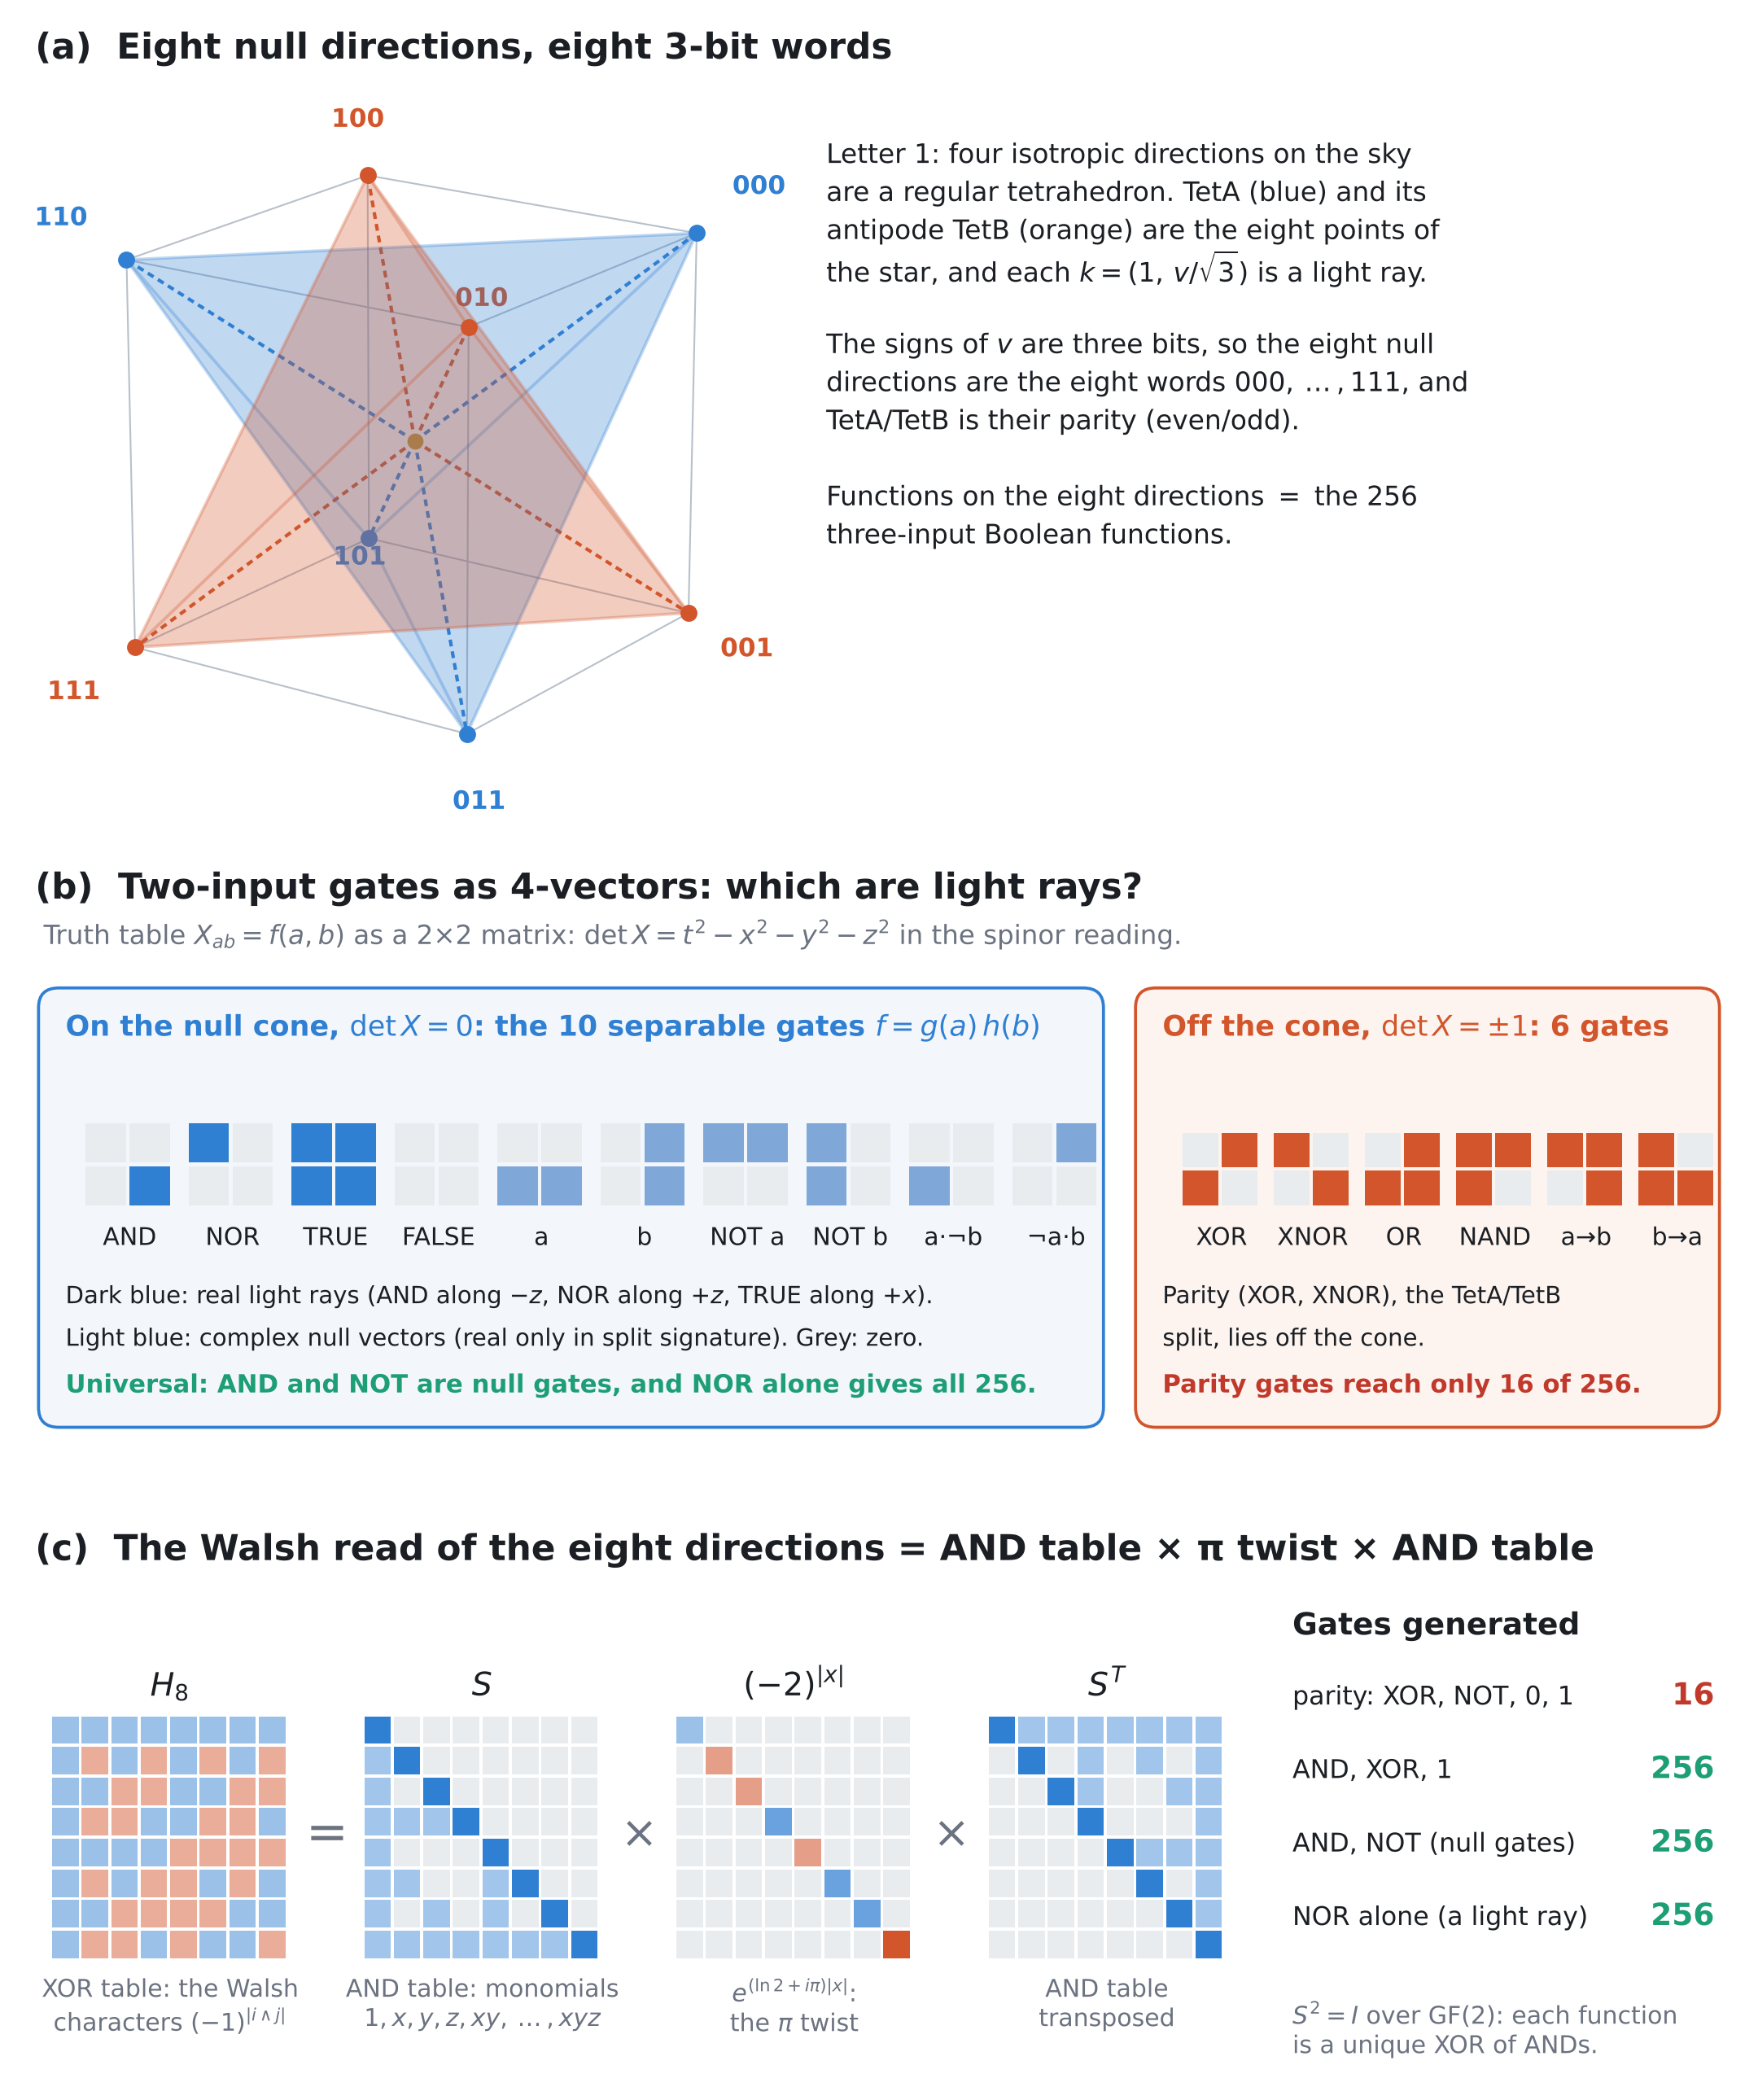
\includegraphics[width=0.84\textwidth]{null_cone_boolean_figure.png}
\caption{(a) The eight null directions of the tetrad frame (Letter~1),
labelled by the signs of their spatial parts: the eight three-bit
words, with TetA and TetB the even and odd words. (b) The $16$
two-input gates, with truth tables read as $2\times2$ matrices $X$. In
the spinor reading $\det X$ is the Minkowski norm. Ten gates are null,
the separable gates $g(a)h(b)$; AND, NOR and TRUE are real light rays.
The other six, including parity, are off the cone (Theorem~3).
(c) The Walsh read of the eight directions factors as an AND table,
a half-turn per bit, and the transposed AND table (Theorem~2). Right:
the number of three-input functions each gate set generates.}
\label{fig:main}
\end{figure*}

% ----------------------------------------------------------------------

\section{The Eight Null Directions}

\paragraph{Proposition 1.} \textit{In a Lorentzian frame, let
$u_1,\dots,u_4$ be unit spatial vectors with zero centroid and
isotropic second moment, so that each $k_I = (1, u_I)$ is null. Then
the $u_I$ are a regular tetrahedron, with $u_I\cdot u_J = -\tfrac13$,
and up to rotation they are $v/\sqrt3$ for the four corners
$v \in \{\pm1\}^3$ with $v_1v_2v_3 = +1$ (TetA). With their antipodes
(TetB) they are the eight corners of the cube. Writing each corner's
signs as bits, $b_i = (1 - v_i)/2$, the eight null directions are the
eight words $b \in \{0,1\}^3$, and TetA and TetB are the words of even
and odd weight.}

\paragraph{Proof.} The tetrahedron is Letter~1's
proposition~\cite{NelsonL1}; squaring the centroid condition gives
$4 + 12c = 0$. The rest is the substitution $v_i = (-1)^{b_i}$, under
which $v_1v_2v_3 = (-1)^{|b|}$. \hfill $\square$

\medskip
\noindent
So a function on the eight null directions is exactly a three-input
Boolean function, and there are $2^8 = 256$ of them.

% ----------------------------------------------------------------------

\section{Representation Versus Gates}

Let $H_8$ have entries $(-1)^{|i \wedge j|}$, the Walsh characters of
the cube~\cite{Walsh1923,Sylvester1867}, where $i \wedge j$ is the
bitwise AND of the words and $|\cdot|$ counts ones.

\paragraph{Proposition 2 (representation).} \textit{$H_8^2 = 8I$, so
every function on the eight null directions is a unique real
combination of the eight Walsh characters.}

\medskip
\noindent
This is the sense of the archive's claim, and it is generic: the same
holds for any eight labelled points. It says nothing about which gates
the structure supplies. The Walsh characters themselves are, in $0/1$
form, the parities $x_J = \bigoplus_{i\in J} b_i$.

\paragraph{Theorem 1 (parity is not universal).} \textit{Every Walsh
character, and the TetA/TetB indicator, is affine over GF(2): its
algebraic normal form has degree at most one. Closing the three
projections under XOR, NOT and the constants gives exactly the $16$
affine functions of three bits, not all $256$. So no set of parity
gates is universal.}

\paragraph{Proof.} A parity is a sum of variables over GF(2), and
compositions of affine functions are affine. The count of $16$ is
checked by exhaustive closure. By Post's theorem~\cite{Post1941} a
gate set inside the affine class is not functionally complete.
\hfill $\square$

\medskip
\noindent
In particular the XOR read off the octahedral node's grade-two Walsh
coefficient, and the parity term it reads at grade three, are affine.
The node computes NAND and the full adder because its readout is a
real linear combination of Walsh coefficients, which is
Proposition~2, not because parity gates are universal.

% ----------------------------------------------------------------------

\section{The Walsh Read Factors Into AND and XOR}

Let $S$ be the $8 \times 8$ matrix with $S_{ij} = 1$ when the bits of
$j$ are a subset of those of $i$, and $0$ otherwise. Equivalently,
$S = A^{\otimes 3}$ with
$A = \bigl(\begin{smallmatrix}1&0\\1&1\end{smallmatrix}\bigr)$, the
Sierpi\'nski triangle.

\paragraph{Theorem 2.} \textit{(i) $S_{ij}$ is the AND of the bits of
$j$ at the corner $i$: $S$ is the evaluation table of the eight AND
monomials $1, x, y, z, xy, xz, yz, xyz$. (ii) $S^2 = I$ over GF(2), so
every Boolean function is a unique XOR of AND monomials, its algebraic
normal form, with coefficients $S f \bmod 2$. (iii)}
\begin{equation}
  H_8 = S\,D\,S^T, \qquad
  D = \mathrm{diag}\big((-2)^{|x|}\big) = e^{(\ln 2 + i\pi)|x|} .
\end{equation}
\textit{(iv) AND, XOR and the constant $1$ generate all $256$
functions.}

\paragraph{Proof.} (i) A monomial $\prod_{b \in J} x_b$ is $1$ at a
corner exactly when every bit of $J$ is set there. (ii) $A^2 \equiv I
\pmod 2$, and tensor powers follow. This is the Zhegalkin, or
Reed--Muller, expansion~\cite{Zhegalkin1927,Muller1954}. (iii) Entry
by entry, with $n = |i \wedge j|$,
$\sum_{K \subseteq i \wedge j} (-2)^{|K|} = (1 - 2)^n = (-1)^n$.
(iv) follows from (ii), and is also checked by exhaustive closure.
\hfill $\square$

\medskip
\noindent
So the Walsh read of the eight null directions factors into the two
halves of a universal gate set. The outer factors are the AND table;
the half-turn $e^{i\pi}$ per bit in the middle carries the parity
signs. The universality of the structure is located in the
Sierpi\'nski factor, not in the Hadamard sign pattern. In the spinor
reading of the next section, $A$ acting on both indices is a null
rotation~\cite{NelsonNullRot}.

% ----------------------------------------------------------------------

\section{The Null Cone of the Two-Bit Block}

Write a two-input gate as its truth table $X_{ab} = f(a,b)$, a
$2\times2$ matrix, and read the two bits as the two spinor indices of a
$4$-vector, $X = t + x\sigma_1 + y\sigma_2 + z\sigma_3$, so that
$\det X = t^2 - x^2 - y^2 - z^2$~\cite{PenroseRindler}. This is the
reading in which the tetrad frame's legs form a Newman--Penrose null
tetrad~\cite{NelsonNullRot}.

\paragraph{Theorem 3 (the null gates).} \textit{A gate is null,
$\det X = 0$, exactly when $X$ has rank at most one, that is, when
$f(a,b) = g(a)\,h(b)$. Exactly $10$ of the $16$ gates are null: FALSE,
TRUE, AND, NOR, the four literals $a$, $b$, $\neg a$, $\neg b$, and
$a\wedge\neg b$, $\neg a \wedge b$. The other six, XOR, XNOR, OR, NAND
and the two implications, have $\det X = \pm1$. Among the null gates,
AND, NOR and TRUE are real light rays, along $-z$, $+z$ and $+x$;
FALSE is the zero vector; the remaining six are complex null vectors,
real only in the split-signature reading of real $2\times2$ matrices.
AND is the light ray $|11\rangle$ fixed by the Sierpi\'nski null
rotation $X \mapsto AXA^T$.}

\paragraph{Proof.} A $2\times2$ matrix is singular exactly when its
rank is at most one, and a $0/1$ matrix of rank one is an outer
product $g\,h^T$ of $0/1$ vectors. The components follow from
$x^\mu = \tfrac12\mathrm{Tr}(\sigma_\mu X)$; a non-symmetric $X$ has
an imaginary $y$ component. $A$ fixes $|1\rangle$. \hfill $\square$

\paragraph{Corollary.} \textit{The null gates are a universal set:
they contain AND and NOT. NOR, a real light ray, is universal on its
own. Parity, XOR and XNOR, lies off the cone.}

\paragraph{Proof.} $\{\mathrm{AND}, \mathrm{NOT}\}$ and $\{\mathrm{NOR}\}$
are classical complete sets~\cite{Post1941,Sheffer1913}; exhaustive
closure confirms that each generates all $256$ three-input functions.
\hfill $\square$

\medskip
\noindent
Rank-one truth tables are the combinatorial rectangles of
communication complexity~\cite{Kushilevitz1997}; the observation here is
that, in the spinor reading of the frame, they are its light rays.

% ----------------------------------------------------------------------

\section{Discussion and Scope}

The archive's claim, that the null cone of the frame is a universal
Boolean operator, is true in two senses, and they should be kept
apart. In the weak sense, representation, it holds for the eight null
directions as for any eight labelled points (Proposition~2). In the
strong sense, functional completeness, it holds in a specific way.
Parity alone, the structure that separates TetA from TetB, is not
universal (Theorem~1). The Walsh read of the eight directions factors
into an AND table and a half-turn (Theorem~2), and on the two-bit
block the light rays are exactly the separable gates, which are
universal, while parity is off the cone (Theorem~3).

What is standard and what is new: Post's theorem, the algebraic normal
form, the completeness of NOR, and the spinor--vector correspondence
are classical. The new content is their placement on the frame: the
null directions as the three-bit words, the factorisation of their
Walsh read into AND and XOR tables, and the identification of the
separable gates with the light rays of the spinor reading.

The paper does not show that physical light computes, nor that a
lattice of photons is a computing medium; those remain the archive's
interpretation. The real form matters: only AND, NOR and TRUE are real
light rays in Minkowski signature, and the other null gates are real
only in split signature. The ten null and six non-null gates should
not be confused with the archive's split of $16$ into $10$ symmetric
and $6$ antisymmetric components: the null gates do not form a linear
subspace, and no relation between the two counts is claimed.

Every statement is checked by the accompanying script (18 checks,
exact arithmetic, closures exhaustive over all $256$ functions).

% ----------------------------------------------------------------------

\begin{thebibliography}{99}

\bibitem{NelsonL1}
S.~Nelson,
\textit{The Coordinate-Space Geometry of the Tetrad Frame}, Letter~1
(2026), with the supplement \textit{From the Lorentz signature to the
tetrahedral frame}.

\bibitem{NelsonPixel}
S.~Nelson,
\textit{The universe is pixelated} (2026), research archive,
\texttt{universe-is-pixelated/}.

\bibitem{NelsonNullRot}
S.~Nelson,
\textit{G's graded operator is a null rotation} (2026),
\texttt{proofs/g-null-rotation/}.

\bibitem{Post1941}
E.~L.~Post,
\textit{The Two-Valued Iterative Systems of Mathematical Logic},
Annals of Mathematics Studies~5 (Princeton University Press, 1941).

\bibitem{Zhegalkin1927}
I.~I.~Zhegalkin,
``On the technique of calculating propositions in symbolic logic'',
\textit{Mat. Sb.} \textbf{34} (1927) 9--28.

\bibitem{Muller1954}
D.~E.~Muller,
``Application of Boolean algebra to switching circuit design and to
error detection'', \textit{IRE Trans. Electron. Comput.}
\textbf{EC-3} (1954) 6--12.

\bibitem{Sheffer1913}
H.~M.~Sheffer,
``A set of five independent postulates for Boolean algebras, with
application to logical constants'', \textit{Trans. Amer. Math. Soc.}
\textbf{14} (1913) 481--488.

\bibitem{Walsh1923}
J.~L.~Walsh,
``A closed set of normal orthogonal functions'',
\textit{Amer. J. Math.} \textbf{45} (1923) 5--24.

\bibitem{Sylvester1867}
J.~J.~Sylvester,
``Thoughts on inverse orthogonal matrices'',
\textit{Phil. Mag.} \textbf{34} (1867) 461--475.

\bibitem{PenroseRindler}
R.~Penrose and W.~Rindler,
\textit{Spinors and Space-Time}, vol.~1
(Cambridge University Press, 1984).

\bibitem{Kushilevitz1997}
E.~Kushilevitz and N.~Nisan,
\textit{Communication Complexity}
(Cambridge University Press, 1997).

\end{thebibliography}

\end{document}
